% Architectuur 1 blz
\chapter{Architectuur}\label{chapter:architectuur}

%%%%%%%%%%%%%%%%%%
% SECTION
%%%%%%%%%%%%%%%%%%
\section{Verzamelen van data}\label{section:manuele_datainvoer}

Om relatief snel een applicatie te kunnen implementeren, werd in de applicatie eerst manuele datainvoer voorzien.

Het aanvankelijke idee om gebruik te maken van de Toggle API\footnote{\url{https://www.toggl.com/public/api}} is uiteindelijk niet meer ge\"implementeerd. Indien de gebruik zou gemaakt worden van de Toggl API zou er natuurlijk een internetconnectie moeten opgezet worden. De gebruiker zou zich moeten authenticeren, waarna logingegevens in lokaal zouden kunnen bijgehouden worden en dergelijke.


%%%%%%%%%%%%%%%%%%
% SECTION
%%%%%%%%%%%%%%%%%%
\section{Opslag van data}\label{section:local_storage}

De applicatie maakt gebruik van lokale opslag om gegevens te persisteren. De records bevatten relatief beperkte, numerieke informatie. De huidige smartphones hebben gemakkelijk meer dan een gigabyte aan intern geheugen\cite{schiesser2012}, dus de gebruiker zou al duizenden records moeten opslaan vooraleer een significant deel van de opslagcapaciteit zou gebruikt worden. Daarnaast heeft lokale opslag het voordeel dat het een hogere beschikbaarheid aanbiedt dan opslag op een externe server. Ten slotte is externe, online opslag geen vereiste om resultaten te verkrijgen die significant zijn. Uiteraard kan het vergelijken met andere gebruikers, gemiddeldes en uitschieters een interessante uitbreiding zijn bij de data-analyse.

De interne architectuur van de applicatie is afgebeeld op figuur \ref{fig:architecture}.

\begin{figure}
  \begin{center}
  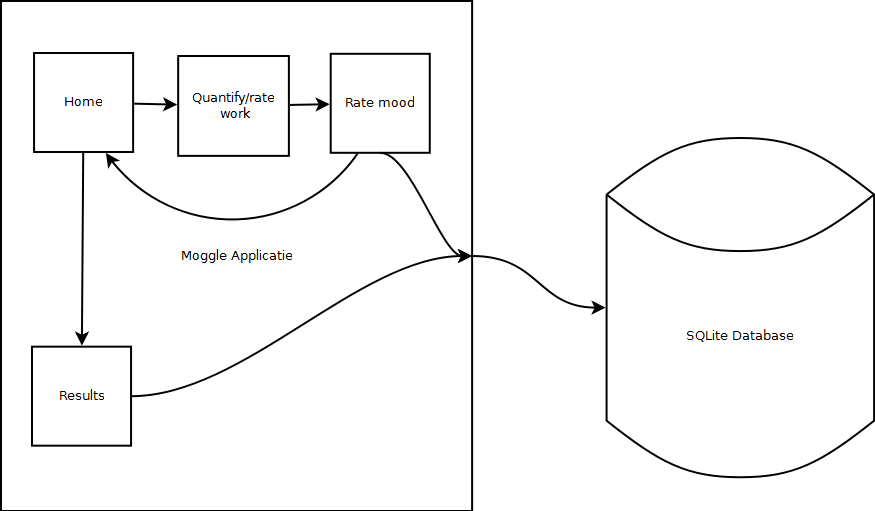
\includegraphics[scale=0.35]{data/internal-architecture}
	\end{center}
  \caption{Interne architectuur van de Moggle applicatie}
  \label{fig:architecture}
\end{figure}

%Een cli\"ent-server model 




